% This must be in the first 5 lines to tell arXiv to use pdfLaTeX, which is strongly recommended.
\pdfoutput=1
% In particular, the hyperref package requires pdfLaTeX in order to break URLs across lines.

\documentclass[11pt]{article}
\usepackage{tabularx}
\usepackage{booktabs}
\usepackage{float}
\usepackage[colorinlistoftodos, textsize=tiny]{todonotes}

\usepackage[utf8]{inputenc}
\usepackage{listings}
\usepackage{xcolor}

\lstdefinestyle{mypython}{
  language=Python,
  basicstyle=\ttfamily\small,
  keywordstyle=\color{blue},
  stringstyle=\color{green!40!black},
  commentstyle=\color{gray},
  showstringspaces=false,
  frame=single,
  breaklines=true,
  tabsize=2
}

% Change "review" to "final" to generate the final (sometimes called camera-ready) version.
% Change to "preprint" to generate a non-anonymous version with page numbers.
\usepackage[preprint]{acl}
\usepackage{booktabs}
% Standard package includes
\usepackage{times}
\usepackage{latexsym}

% For proper rendering and hyphenation of words containing Latin characters (including in bib files)
\usepackage[T1]{fontenc}
% For Vietnamese characters
% \usepackage[T5]{fontenc}
% See https://www.latex-project.org/help/documentation/encguide.pdf for other character sets

% This assumes your files are encoded as UTF8
\usepackage[utf8]{inputenc}
\lstset{
  basicstyle=\ttfamily,
  columns=fullflexible,
  keepspaces=true,
  frame=single
}


% This is not strictly necessary, and may be commented out,
% but it will improve the layout of the manuscript,
% and will typically save some space.
\usepackage{microtype}

% This is also not strictly necessary, and may be commented out.
% However, it will improve the aesthetics of text in
% the typewriter font.
\usepackage{inconsolata}

%Including images in your LaTeX document requires adding
%additional package(s)
\usepackage{graphicx}

% If the title and author information does not fit in the area allocated, uncomment the following
%
%\setlength\titlebox{<dim>}
%
% and set <dim> to something 5cm or larger.

\title{AI-Generated Text Detection with SVM and LoRA-Finetuned RoBERTa}

% Author information can be set in various styles:
% For several authors from the same institution:
% \author{Author 1 \and ... \and Author n \\
%         Address line \\ ... \\ Address line}
% if the names do not fit well on one line use
%         Author 1 \\ {\bf Author 2} \\ ... \\ {\bf Author n} \\
% For authors from different institutions:
% \author{Author 1 \\ Address line \\  ... \\ Address line
%         \And  ... \And
%         Author n \\ Address line \\ ... \\ Address line}
% To start a separate ``row'' of authors use \AND, as in
% \author{Author 1 \\ Address line \\  ... \\ Address line
%         \AND
%         Author 2 \\ Address line \\ ... \\ Address line \And
%         Author 3 \\ Address line \\ ... \\ Address line}

\author{
\begin{tabular}{cc}
Marie Yang\textsuperscript{1}\textsuperscript{*} & Harris Song\textsuperscript{1}\textsuperscript{*} \\
\texttt{marieyang@ucla.edu} & \texttt{harris.song@ucla.edu} \\
\\ % Blank line for spacing
Anish Pal\textsuperscript{1}\textsuperscript{*} & Aditya Patil\textsuperscript{1}\textsuperscript{*} \\
\texttt{anishmpal@ucla.edu} & \texttt{adityapatil@ucla.edu}
\end{tabular}
\\
\textsuperscript{1}Department of Computer Science \\
University of California, Los Angeles \\
$^{*}$ \textit{Denotes Equal Contribution}
}

\begin{document}
\maketitle
\section{Introduction}


As large language models (LLMs) like ChatGPT and Claude become increasingly capable and accessible, AI-generated content is rapidly flooding the internet. While these tools have many beneficial applications, they also bring about significant issues, including the spread of misinformation and hallucinations.  \cite{xu2024inevitable}. Given the limitations of existing detectors, our goal was to build a more robust and reliable classifier. We trained a traditional Support Vector Machine as a baseline and fine-tuned RoBERTa, a widely used BERT variant, using Low-Rank Adaptation on the HC3 dataset. 


\section{Modeling Approach}
In this section, we outline our modeling strategy for text classification. We begin with a classical baseline presented in \autoref{sec:intro_svm}, then progressively adopt more sophisticated neural methods in \autoref{sec:intro_roberta} and \autoref{sec:intro_lora}; this comparative approach allows us to quantify the improvements gained from recent advancements in language modeling and parameter-efficient fine-tuning.
\subsection{Support Vector Machine (SVM)}
\label{sec:intro_svm}
For our baseline model, we used a support vector machine (SVM), a classical machine learning technique \cite{cortes1995support}. We compared this approach with a more complex, attention-based approach to see what benefits it would yield in comparison and will discuss this in \autoref{svm_results}.


\subsection{Finetuning RoBERTa}
\label{sec:intro_roberta}
We fine-tuned an encoder-only model, RoBERTa \cite{liu2020roberta}, which is a robustly optimized variant of BERT that significantly outperforms BERT on a number of metrics. For the full model architecture, refer to \autoref{fig:architecture}. We also considered variants such as DeBERTa \cite{he2021deberta}, which adds a decoder mask on top of BERT and a better attention mechanism. 

Upon further research on existing text classifiers, we found OpenAI's RoBERTa GPT-2 generated text detector \cite{openai_roberta_detector} that was released alongside the GPT-2 XL model and fine-tuned on GPT-2 text data. We decided against fine-tuning OAI's existing classifier, however, given that we saw no improvement in accuracy from the OAI baseline of about 87\% after some initial training. Instead, we ultimately chose to train RoBERTa base on our own training data.

\subsection{Low Rank Adaptation}
\label{sec:intro_lora}
\begin{figure*}[ht]
  \centering
  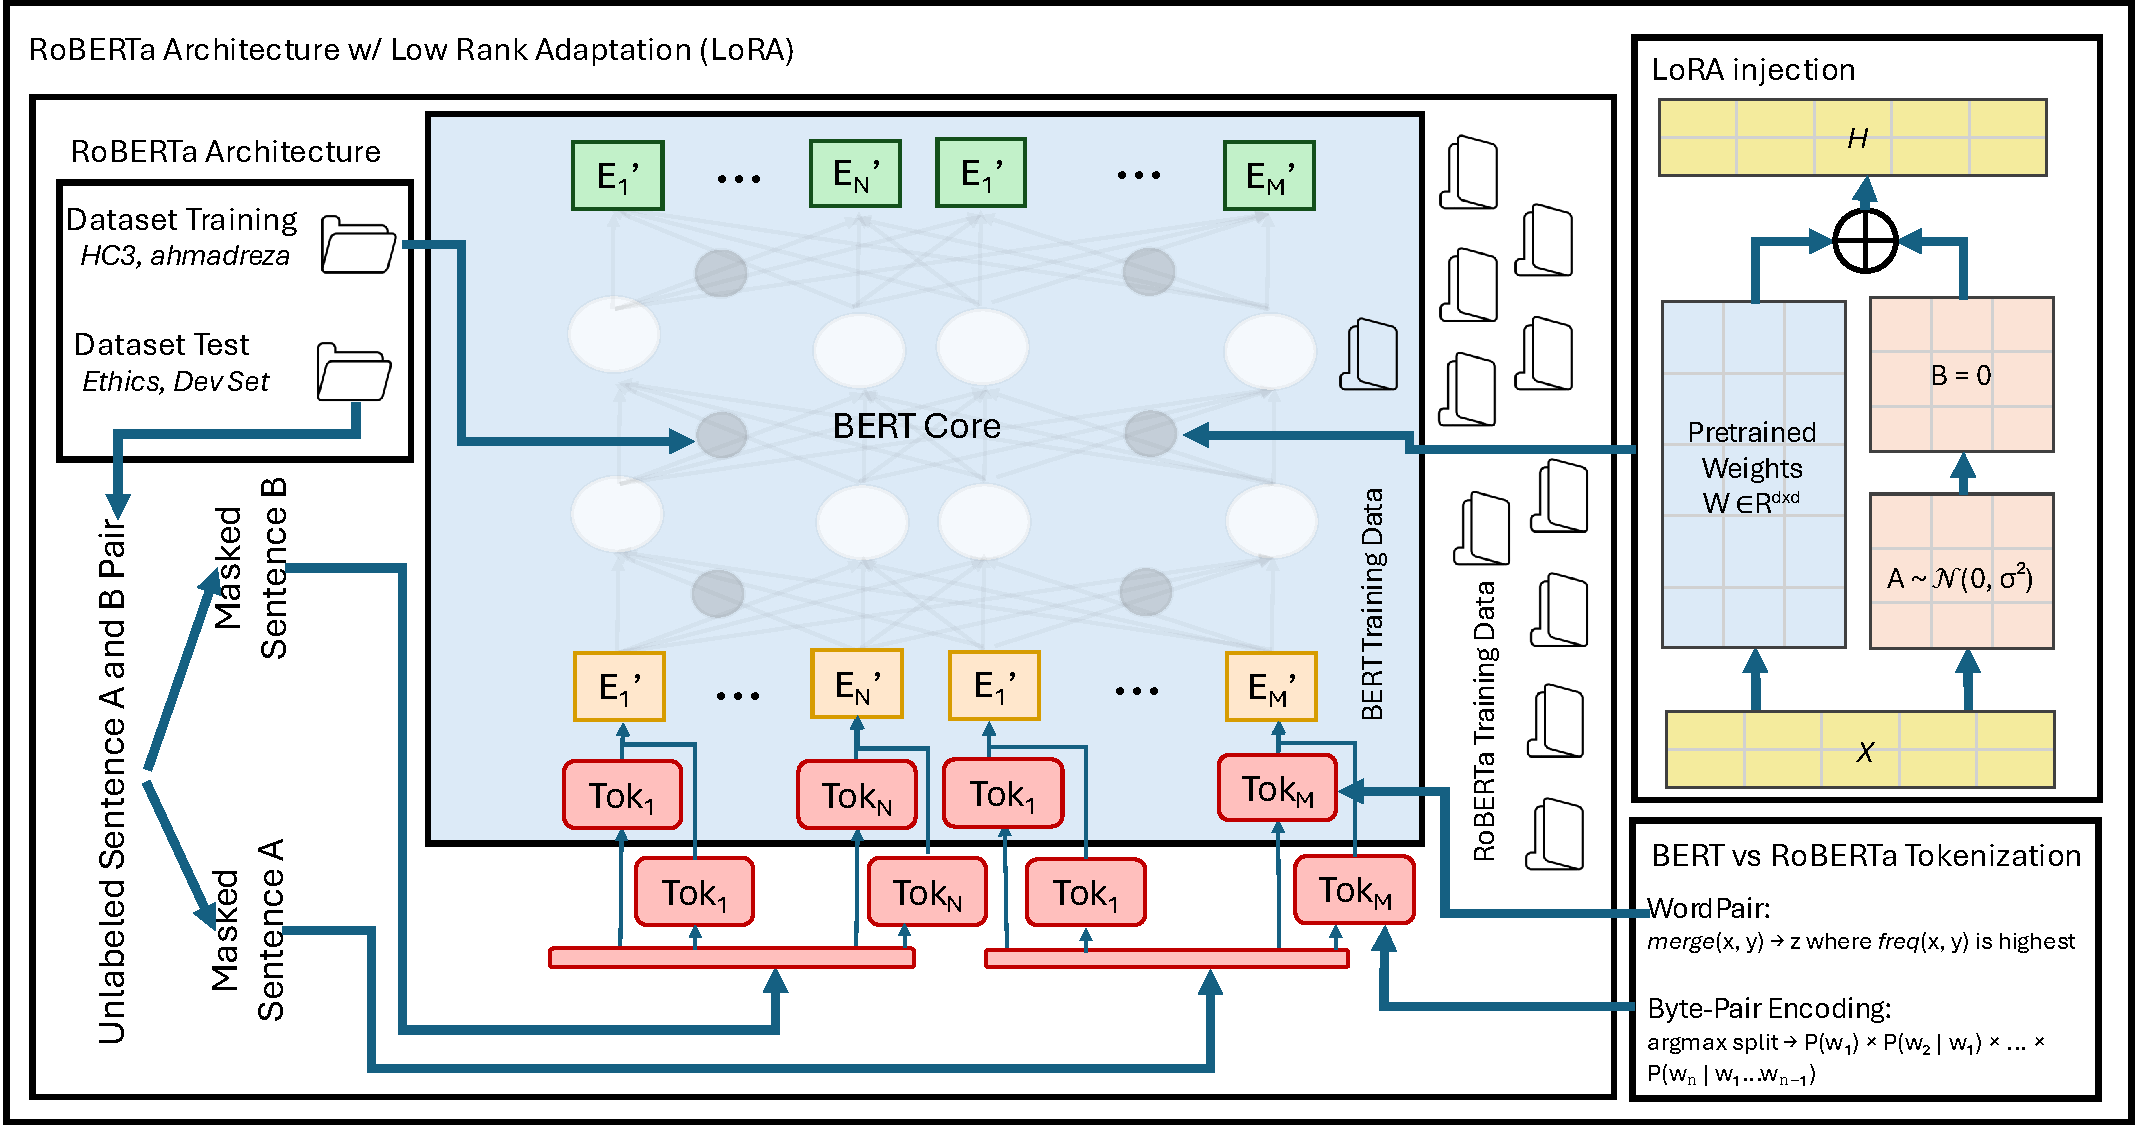
\includegraphics[width=\textwidth]{Final-Paper/tables-and-figures/architecture.pdf}
    \caption{Our architecture w/ Training and Test dataset, including the baseline BERT \cite{devlin2019bert}, RoBERTa \cite{liu2020roberta}, and LoRA \cite{hu2021lora}}
  \label{fig:architecture}
\end{figure*}


To improve accuracy and reduce training time and compute, we used Low Rank Adaptation (LoRA) \cite{hu2021lora}, shown in \autoref{fig:architecture} to train our model. LoRa freezes the pre-trained weights of the RoBERTa model and inserts low-rank trainable adapters between certain layers. These adapters are small matrices that allow efficient fine-tuning with far fewer parameters and training time, while maintaining performance.

\begin{figure}[H]
    \centering
    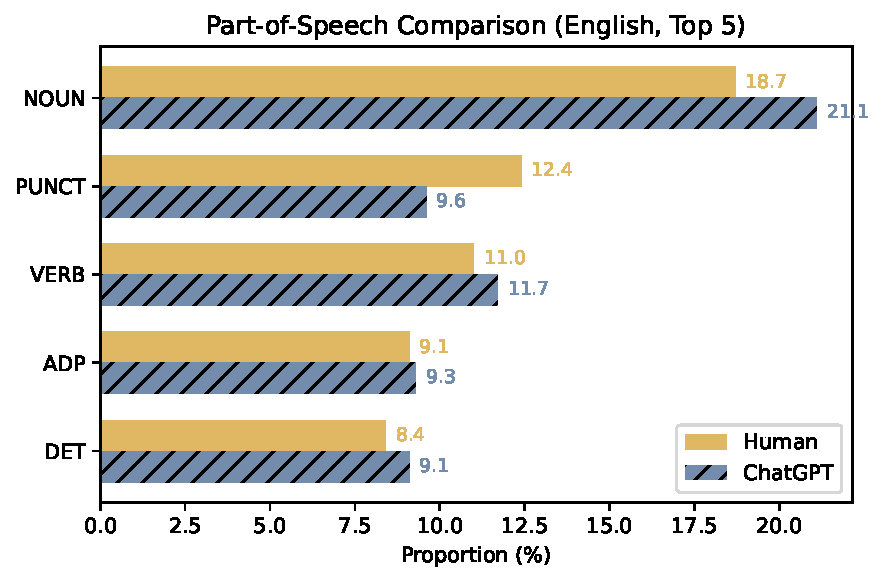
\includegraphics[width=\columnwidth]{Final-Paper/tables-and-figures/pos_comparison_en_top5.pdf}
    \caption{POS Comparison \cite{marcus1993building} from the HC3 Dataset \cite{guo2023hc3}}
    \label{fig:data-pdf}
\end{figure}



\section{Dataset Collection}
\label{sec:dataset}
\vspace{-2mm}


We initially trained on ahmadreza13's 3.6 million-sample dataset on HuggingFace \cite{ahmadreza13_human_vs_Ai_generated_dataset}. Fine-tuning base RoBERTa on this dataset resulted in extremely poor performance with an accuracy of 0.457. This dataset had no explicit comparison between human and AI-generated texts for the same prompt, and we felt there were higher quality datasets available. Therefore, we chose to switch to the \textbf{HC3 dataset} \cite{guo2023hc3}.






The \textbf{HC3 (Human ChatGPT Comparison Corpus)} dataset is a practical and well-structured database used for analyzing differences between human-written and ChatGPT-generated text. The English portion of the dataset contains roughly 24,300 question–answer pairs, covering five main domains: Reddit Explain Like I’m 5 (ELI5) ($\sim$17,000 examples), finance ($\sim$3,900), medicine ($\sim$1,250), open-domain QA ($\sim$1,190), and computer science/artificial intelligence wiki questions ($\sim$840). Each example consists of a question, one or more human-written responses, and one or more responses generated by ChatGPT. 

In addition to its breadth of content, the dataset also exhibits valuable structural patterns which can inform model development. For example, ChatGPT responses generally tend to be longer and more formally structured, often including introductory phrases and carefully worded explanations, while human responses are typically more concise and stylistically varied. In the finance and medicine subsets, human responses frequently reference external knowledge or personal anecdotes, while ChatGPT tends to produce more generalized and less polarizing answers.  Stylistically, ChatGPT answers include redundant phrasing or cautionary disclaimers, especially in sensitive domains such as medicine and law.





\section{Hyperparameters}

We used the following hyperparameters for finetuning roberta-base with LoRA:
\begin{lstlisting}[style=mypython, caption={LoRA Configuration}]
lora_config = LoraConfig(
    r=8,
    lora_alpha=16,
    target_modules=["query", "value"],  # Commonly targeted layers
    lora_dropout=0.1,
    bias="none",
    task_type=TaskType.SEQ_CLS
)
\end{lstlisting}

\begin{lstlisting}[style=mypython, caption={Training Arguments}]
training_args = TrainingArguments(
    output_dir=output_dir,
    eval_strategy="epoch",
    save_strategy="epoch",
    per_device_train_batch_size=8,
    per_device_eval_batch_size=8,
    num_train_epochs=3,
    label_names=["labels"], 
    weight_decay=0.01,
    logging_steps=50,
    load_best_model_at_end=True,
    metric_for_best_model="accuracy",
    save_total_limit=2,
    resume_from_checkpoint=True if os.path.exists(output_dir) else False)
\end{lstlisting}

\section{Results}
\subsection{Support Vector Machine Baseline}
\label{svm_results}
Training an SVM on our dataset resulted in a decent performance baseline with an accuracy of $\sim$70\%. 

\begin{table}[H]
\centering
\caption{SVM Classification Report}
\label{tab:svm_table}
\resizebox{\columnwidth}{!}{%
\begin{tabular}{lcccc}
\toprule
\textbf{Class} & \textbf{Precision} & \textbf{Recall} & \textbf{F1-score} & \textbf{Support} \\
\midrule
AI (0) & 0.69 & 0.70 & 0.70 & 12,000 \\
Human (1)    & 0.70 & 0.69 & 0.70 & 12,000 \\
\midrule
\textbf{Accuracy}     &       &       & \textbf{0.70} & 24,000 \\
\textbf{Macro Avg}    & 0.70  & 0.70  & 0.70           & 24,000 \\
\textbf{Weighted Avg} & 0.70  & 0.70  & 0.70           & 24,000 \\
\bottomrule
\end{tabular}%
}
\end{table}


\begin{figure}[H]
    \centering
    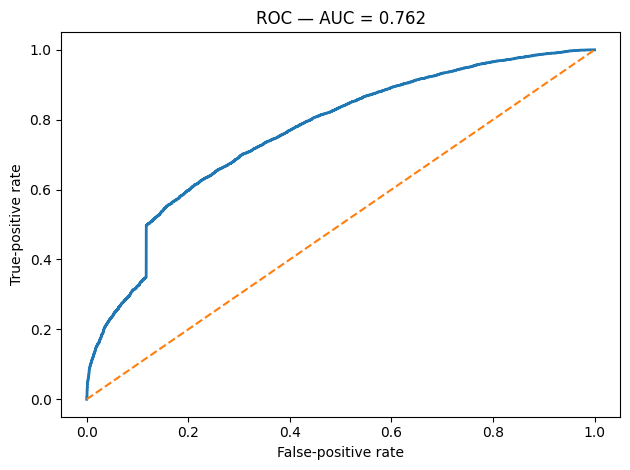
\includegraphics[width=1\linewidth]{Final-Paper/tables-and-figures/svm_roc.png}
    \caption{SVM ROC-AUC Curve}
    \label{fig:svm_roc}
\end{figure}


Our AUC-ROC \cite{hanley1982meaning} curve for our SVM at \autoref{fig:svm_roc}.
Area under the curve being 0.762 suggests that the SVM model has a moderate ability to discriminate between AI and human-written text.
\subsection{Finetuned RoBERTa}
\label{sec:roberta_finetuning}
Fine-tuning with LoRA on 48,644 data points in the HC3 dataset gave us a  model accuracy of 92\% over the entire development set (excluding the ethics dev set).

\begin{table}[H]
\centering
\caption{Finetuned RoBERTa Classification Report for Entire Dev Set}
\label{tab:entire_dataset}
\resizebox{\columnwidth}{!}{%
\begin{tabular}{lcccc}
\toprule
\textbf{Class} & \textbf{Precision} & \textbf{Recall} & \textbf{F1-score} & \textbf{Support} \\
\midrule
AI (0) & 0.8994 & 0.9392 & 0.9189 & 12,000 \\
Human (1) & 0.9364 & 0.8950 & 0.9152 & 12,000 \\
\midrule
\textbf{Accuracy}     &        &        & \textbf{0.9171} & 24,000 \\
\textbf{Macro Avg}    & 0.9179 & 0.9171 & 0.9170 & 24,000 \\
\textbf{Weighted Avg} & 0.9179 & 0.9171 & 0.9170 & 24,000 \\
\bottomrule
\end{tabular}%
}
\end{table}

We can see from the table that our model has slightly higher precision for the Human (1) class and higher recall for the AI (0) class. This implies that when the model predicts a text to be human-generated, it is likely to be correct, but it may miss some human examples. On the other hand, the model catches most AI-generated texts, but mistakenly flags some human texts as AI in order to do this. Overall, there is a precision-recall tradeoff where the model errs on the side of classifying some human text as AI in order to catch more AI examples.

This trade-off has significant implications for real-world applications of AI detection systems. On one hand, a model that incorrectly flags human work as AI-generated can lead to serious consequences, such as students being falsely accused of plagiarism. On the other hand, failing to detect AI-generated content could undermine the integrity of educational assessments and allow cheating to go undetected. Therefore, striking a careful balance is essential.

\begin{figure}[H]
    \centering
    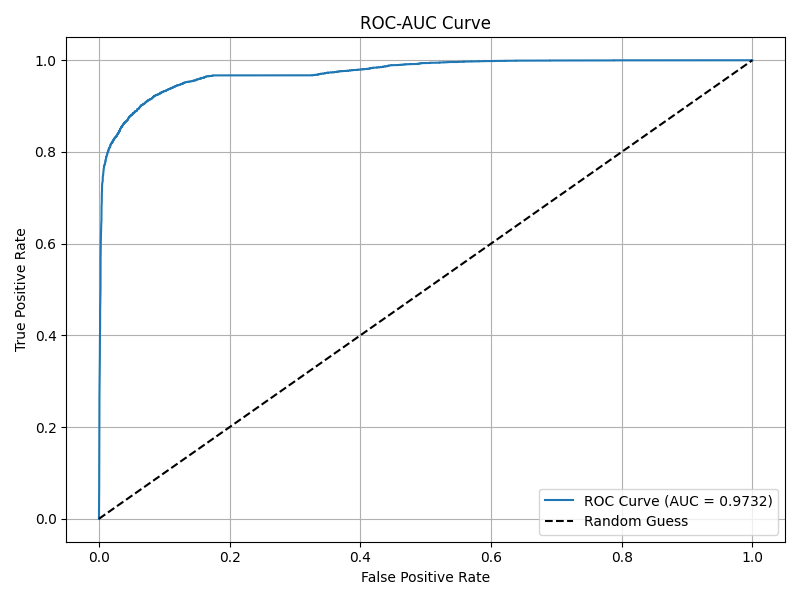
\includegraphics[width=\linewidth]{Final-Paper/tables-and-figures/roc_curve.png}
    \caption{Finetuned RoBERTa ROC-AUC Curve}
    \label{fig:roberta_roc}
\end{figure}
\subsection{Discussion}

Our model had outstanding performance on the arxiv\_chatgpt dataset, achieving an accuracy of 99\%, and lower, relatively similar performances of around 89\% across the other datasets (arxiv\_cohere, reddit\_chatgpt and reddit\_cohere).

This is somewhat surprising. The HC3 dataset consists entirely of ChatGPT-generated text, so we would expect it to perform better on ChatGPT text than Cohere text, which it did. However, a significant portion of the HC3 dataset -- 17.1k out of 24.3k samples, or roughly 70\% -- is made up of text sourced from Reddit. Despite our training dataset being dominated by Reddit text, our model still performs better on  arxiv\_chatgpt than reddit\_chatgpt. 

Our hypothesis for this phenomenon is that Reddit texts are simply inherently harder to classify than arXiv texts. While Reddit texts can vary greatly in tone, content and vocabulary, arXiv papers follow a more uniform academic writing style with consistent technical language. This uniformity may make it easier for the model to detect patterns in the arXiv dataset. Furthermore, the HC3 dataset does still include a significant amount of technical texts in the domains of medicine and computer science/artificial intelligence. \autoref{tab:arxiv_chatgpt}, \autoref{tab:arxiv_cohere}, \autoref{tab:reddit_chatgpt}, and \autoref{tab:reddit_cohere} include our results.

\begin{table}[ht]
\centering
\caption{Report for \texttt{arxiv\_chatGPT.jsonl}}
\label{tab:arxiv_chatgpt}
\resizebox{\columnwidth}{!}{%
\begin{tabular}{l c c c c}
\toprule
\textbf{Class} & \textbf{Precision} & \textbf{Recall} & \textbf{F1-score} & \textbf{Support} \\
\midrule
0 & 1.0000 & 0.9800 & 0.9899 & 3000 \\
1 & 0.9804 & 1.0000 & 0.9901 & 3000 \\
\midrule
\textbf{Accuracy} &       &       & \textbf{0.9900} & 6000 \\
\textbf{Macro Avg} & 0.9902 & 0.9900 & 0.9900 & 6000 \\
\textbf{Weighted Avg} & 0.9902 & 0.9900 & 0.9900 & 6000 \\
\bottomrule
\end{tabular}%
}
\end{table}

\begin{table}[ht]
\centering
\caption{Report for \texttt{arxiv\_cohere.jsonl}}
\label{tab:arxiv_cohere}
\resizebox{\columnwidth}{!}{%
\begin{tabular}{l c c c c}
\toprule
\textbf{Class} & \textbf{Precision} & \textbf{Recall} & \textbf{F1-score} & \textbf{Support} \\
\midrule
0 & 1.0000 & 0.7890 & 0.8821 & 3000 \\
1 & 0.8258 & 1.0000 & 0.9046 & 3000 \\
\midrule
\textbf{Accuracy} &       &       & \textbf{0.8945} & 6000 \\
\textbf{Macro Avg} & 0.9129 & 0.8945 & 0.8933 & 6000 \\
\textbf{Weighted Avg} & 0.9129 & 0.8945 & 0.8933 & 6000 \\
\bottomrule
\end{tabular}%
}
\end{table}

\begin{table}[ht]
\centering
\caption{Report for \texttt{reddit\_chatGPT.jsonl}}
\label{tab:reddit_chatgpt}
\resizebox{\columnwidth}{!}{%
\begin{tabular}{l c c c c}
\toprule
\textbf{Class} & \textbf{Precision} & \textbf{Recall} & \textbf{F1-score} & \textbf{Support} \\
\midrule
0 & 0.8264 & 0.9997 & 0.9048 & 3000 \\
1 & 0.9996 & 0.7900 & 0.8825 & 3000 \\
\midrule
\textbf{Accuracy} &       &       & \textbf{0.8948} & 6000 \\
\textbf{Macro Avg} & 0.9130 & 0.8948 & 0.8937 & 6000 \\
\textbf{Weighted Avg} & 0.9130 & 0.8948 & 0.8937 & 6000 \\
\bottomrule
\end{tabular}%
}
\end{table}

\begin{table}[ht]
\centering
\caption{Report for \texttt{reddit\_cohere.jsonl}}
\label{tab:reddit_cohere}
\resizebox{\columnwidth}{!}{%
\begin{tabular}{l c c c c}
\toprule
\textbf{Class} & \textbf{Precision} & \textbf{Recall} & \textbf{F1-score} & \textbf{Support} \\
\midrule
0 & 0.8247 & 0.9880 & 0.8990 & 3000 \\
1 & 0.9850 & 0.7900 & 0.8768 & 3000 \\
\midrule
\textbf{Accuracy} &       &       & \textbf{0.8890} & 6000 \\
\textbf{Macro Avg} & 0.9049 & 0.8890 & 0.8879 & 6000 \\
\textbf{Weighted Avg} & 0.9049 & 0.8890 & 0.8879 & 6000 \\
\bottomrule
\end{tabular}%
}
\end{table}


\subsection{Error Analysis}
\label{sec:error_analysis}

Our model displayed the ability to distinguish between a human-written paper abstract and a ChatGPT-generated abstract:

\subsection*{LoRA Abstract (Source: LoRA paper)}
\noindent
\textit{"An important paradigm of natural language processing consists of large-scale pre-training on general domain data and adaptation to particular tasks or domains. As we pre-train larger models, full fine-tuning, which retrains all model parameters, becomes less feasible...."} \\
\textbf{Prediction:} Human (1) \quad \textbf{Confidence:} 1.0000

\subsection*{LoRA Abstract (Source: ChatGPT)}
\noindent
\textit{"Low-Rank Adaptation (LoRA) is a parameter-efficient fine-tuning technique for large pre-trained models, particularly transformer-based architectures. Instead of updating all model weights during downstream training, LoRA injects trainable low-rank matrices ..."} \\
\textbf{Prediction:} AI (0) \quad \textbf{Confidence:} 0.9757

However, it was unable to predict some human-generated text that had similar tones and content to what you would expect to see from AI-generated text.

\subsection*{Source: Reddit Dev Set}
\noindent
\textit{"You most likely subscribe to a progressive view of history as a whole, meaning that society advances linearly (populations become more civilized, more knowledgeable, more advanced, etc, essentially superior to those in the past). You most likely believe (implicitly or explicitly) the purpose of history is to define and bolster the nation state..."} \\
\textbf{Prediction:} AI (0), \textbf{True Label:} Human (1) \quad \textbf{Confidence:} 1.0000

\section{Ethics}
\label{sec:ethics}
Our model had lower accuracy on the ethics dev than on the general dev set, but performed almost as well as on the original dev set as it did on the Hewlett dataset as demonstrated at \autoref{tab:hewlett}. Lower performance on the German Wikipedia dataset was expected in \autoref{tab:german_wikipedia}, as the HC3 dataset we used to train had primarily English text, making our model less likely to perform well on datasets that were in a foreign language. This explains why it performed so well on the hewlett dataset, but not the low performance on TOEFL \autoref{tab:toefl}. This could have been due to the fact that for TOEFL, people are required to speak very formally and in less of a casual tone, which the model might have associated with being more similar to AI generated text. 

The performance of our model on these ethics-specific dev sets highlights the importance of textual diversity in training models. With an internet overrun by English text, it's still important to recognize that many other languages are out there, and that they're vastly underrepresented in model training; this makes it so that many models are biased towards English.
\begin{table}[ht]
\centering
\caption{Report for \texttt{hewlett.json}}
\label{tab:hewlett}
\resizebox{\columnwidth}{!}{%
\begin{tabular}{l c c c c}
\toprule
\textbf{Class} & \textbf{Precision} & \textbf{Recall} & \textbf{F1-score} & \textbf{Support} \\
\midrule
0 & 1.0000 & 0.9091 & 0.9524 & 88 \\
1 & 0.0000 & 0.0000 & 0.0000 & 0 \\
\midrule
\textbf{Accuracy} &       &       & \textbf{0.9091} & 88 \\
\textbf{Macro Avg} & 0.5000 & 0.4545 & 0.4762 & 88 \\
\textbf{Weighted Avg} & 1.0000 & 0.9091 & 0.9524 & 88 \\
\bottomrule
\end{tabular}%
}
\end{table}


\begin{table}[ht]
\centering
\caption{Report for \texttt{german\_wikipedia.jsonl}}
\label{tab:german_wikipedia}
\resizebox{\columnwidth}{!}{%
\begin{tabular}{l c c c c}
\toprule
\textbf{Class} & \textbf{Precision} & \textbf{Recall} & \textbf{F1-score} & \textbf{Support} \\
\midrule
0 & 0.5325 & 0.9820 & 0.6906 & 500 \\
1 & 0.8846 & 0.1380 & 0.2388 & 500 \\
\midrule
\textbf{Accuracy} &       &       & \textbf{0.5600} & 1000 \\
\textbf{Macro Avg} & 0.7086 & 0.5600 & 0.4647 & 1000 \\
\textbf{Weighted Avg} & 0.7086 & 0.5600 & 0.4647 & 1000 \\
\bottomrule
\end{tabular}%
}
\end{table}

\begin{table}[ht]
\centering
\caption{Report for \texttt{toefl.json}}
\label{tab:toefl}
\resizebox{\columnwidth}{!}{%
\begin{tabular}{l c c c c}
\toprule
\textbf{Class} & \textbf{Precision} & \textbf{Recall} & \textbf{F1-score} & \textbf{Support} \\
\midrule
0 & 1.0000 & 0.4176 & 0.5891 & 0 \\
1 & 0.0000 & 0.0000 & 0.0000 & 91 \\
\midrule
\textbf{Accuracy} &       &       & \textbf{0.4176} & 91 \\
\textbf{Macro Avg} & 0.5000 & 0.2088 & 0.2946 & 91 \\
\textbf{Weighted Avg} & 1.0000 & 0.4176 & 0.5891 & 91 \\
\bottomrule
\end{tabular}%
}
\end{table}



\section{Related Work}
\label{sec:related_work}

We included related works, and further directions where time constraints and computational bottlenecks are not significant. \cite{gururangan-etal-2020-dont} is an analysis on how domain-adaptive pretraining, such as pretraining within biomedical fields, or in mechanical engineering, is still useful;  future ideas including domain-specific writing styles to identify patterns of authorship. \cite{jiao-etal-2021-self} introduces another interesting approach, discussing translation between languages. Fine-tuning techniques from the language translation (German, Chinese, and English) would be useful in edge cases. 

Lastly, \cite{mitchell2023detectgptzeroshotmachinegeneratedtext} is a paper that uses a novel approach to analyze probabilities. We are also able to graph some of the logit-probabilities through the Transformers package \cite{wolf-etal-2020-transformers}; a benefit includes a lack of fine-tuning due to a more probabilistic approach rather than a generative approach. A lot of our approaches in \autoref{sec:roberta_finetuning} and \autoref{svm_results}, are focused on training, \cite{gururangan-etal-2020-dont}, \cite{jiao-etal-2021-self}, and \cite{mitchell2023detectgptzeroshotmachinegeneratedtext}  define theory-based methods.


\section{Conclusion}

Our experiments demonstrate that fine-tuning RoBERTa with Low-Rank Adaptation (LoRA), as discussed in \autoref{sec:intro_roberta}, \autoref{sec:intro_lora}, \autoref{sec:roberta_finetuning}, and modeled with \autoref{fig:architecture} on the HC3 dataset \cite{guo2023hc3} and analyzed in \autoref{fig:data-pdf} leads to a substantial improvement in detecting AI-generated text compared to traditional machine learning approaches such as SVM, which was extensively discussed in \autoref{sec:intro_svm} and tested in \autoref{svm_results}. In \autoref{sec:error_analysis}, we detail specific test cases, and then we performed our experiments on the ethics dataset in \autoref{sec:ethics}. We finally discuss other related work in \autoref{sec:related_work}.



A limitation of our approach is that our model is trained on primarily ChatGPT and Reddit text, clearly established in \autoref{tab:reddit_chatgpt}. As a result, our architecture is achieves better performances compared to text generated by other LLMs such as Gemini or Claude, or sourced elsewhere, such as arXiV as established with \autoref{tab:arxiv_cohere}. We could incorporate multilingual data into our model, such as the HC3 Chinese dataset for inclusivity. \cite{guo-etal-2023-hc3}. 


The LoRA-augmented RoBERTa model achieved an overall accuracy of over 91\% on the primary evaluation set, with especially high precision in distinguishing human from AI text. In comparison, the SVM baseline reached 70\% accuracy, confirming the advantage of transformer-based models for this task.


\appendix
\newpage
\thispagestyle{empty} 
\section{Appendix: Contribution Statement}
Attached is a contribution statement provided by each author, including the technical and non-technical research work conducted. 

Marie Yang: Train RoBERTa base using HC3 dataset, model evaluations on original dev datasets, model visualizations, write Results section

Harris Song: Set up GCP Virtual machine, read papers and write Related Work section, help write and proofread report, create architecture and data diagrams, SVM training and visualizations

Anish Pal: Train OAI RoBERTa classifier using ahmadreza13 dataset, model evaluations on OAI RoBERTa classifier, analyze training datasets and write Data section

Aditya Patil: Finding and preprocessing training datasets, evaluating and analyzing model on ethics dataset, cleaning Github and writing scripts, writing Ethics section
\thispagestyle{empty}
\bibliography{custom}




\appendix
\end{document}